\lecture{7}{2025-03-10}{Espace $ \mathbb{R}^n$ }{}
\chapter{ Espace $ \mathbb{R}^n $}

\subsection{ $ \mathbb{R}^n$ espace vectoriel normé}
\begin{parag}{Définition}
    \begin{definition}
        $ \mathbb{R}^n$ est un ensemble de tout les $n-$ tuples ordonnés de nombre réels.
        \begin{align*}
            \overline{x} = (x_1, \dots, x_n) = \begin{pmatrix}
                x_1 \\
                \vdots \\ x_n
            \end{pmatrix}
        \end{align*}
        
    \end{definition}
Il y a donc toute les propriétés d'un espace vectoriel dont l'addition et l'action scalaire:
\begin{enumerate}
    \item $+ : \overline{x} = (x_1, \dots, x_n), \overline{y} = (y_1, \dots, y_n) \implies \overline{x} + \overline{y} = (x_1 + y_1, \dots, x_n, y_n)$
    \item Multiplication par un nombre réel $ \lambda \in \mathbb{R}$ :
        \begin{align*}
            \overline{x} = (x_1, \dots, x_n) \implies \lambda \cdot \overline{x} = ( \lambda x_1, \dots, \lambda x_n)
        \end{align*}
\end{enumerate}
Et par conséquent, les opérations présentées ci-dessus satisfont:
\begin{itemize}
    \item $( \lambda_1 \lambda_2) \overline{x} = \lambda_1( \lambda_2 \overline{x}) \; \; \forall \overline{x} \in \mathbb{R}^n, \lambda \in \mathbb{R}$
    \item  $ 1 \cdot \overline{x} = \overline{x}$
    \item $( \lambda_1 + \lambda_2) \overline{x} = \lambda_1 \overline{x} + \lambda_2 \overline{x}$
    \item $ \lambda( \overline{x} + \overline{y}) = \lambda \overline{x} + \lambda \overline{y}\; \;  \forall \lambda_1, \lambda_2 \in \mathbb{R}$
    \item $ \lambda ( \overline{x}+ \overline{y}) = \lambda \overline{x} + \lambda \overline{y}\; \; \forall \overline{x}, \overline{y} \in \mathbb{R}^n$
\end{itemize}

\end{parag}

\begin{parag}{Base}
    On a une base canonique:
    \begin{align*}
        \{ \overline{e}_i = (0, 0, \dots, \overbrace{1}^{i}, \dots, 0)\}_{i=1}^n \implies \overline{e}_i \underbrace{\in}_{ \forall i = 1, \dots, n} \mathbb{R}^n
    \end{align*}

    
\end{parag}

    
\begin{parag}{Produit scalaire}
    On introduit le \important{produit scalaire} dans $ \mathbb{R}^n$:
    \begin{definition}
        \begin{align*}
        < \overline{x}, \overline{y}> =  \sum_{i=1}^n x_i y_i = x_1y_1 + \cdots  + x_ny_n
    \end{align*}
    Et par la suite la \important{norme euclidienne}:
    \begin{align*}
        \mid  \mid \overline{x} \mid  \mid  = ( < \overline{x}, \overline{x}>)^{ \frac{1}{2}} = ( \sum_{i=1}^n x_i^2)^{ \frac{1}{2}} \implies \mathbb{R}^n \text{ est un espace vectoriel normé}
    \end{align*}
    \end{definition}
   \begin{subparag}{Propriétés de la norme euclidienne}
       \begin{enumerate}
           \item $ \mid  \mid \overline{x} \mid  \mid \geq 0$ et $ \mid \mid  \overline{x} \mid  \mid  = 0 \implies \overline{x} = (0, 0, \dots, 0)$
           \item $ \overline{x} \in \mathbb{R}^n, \lambda \in \mathbb{R} \implies \mid  \mid  \lambda \cdot \overline{x} \mid  \mid  = \mid  \lambda \mid \cdot \mid  \mid \overline{x} \mid  \mid $
           \item Cauchy-Schwartz: $ \mid < \overline{x}, \overline{y}> \mid \leq \mid \mid \overline{x} \mid \mid \cdot \mid \mid \overline{y} \mid \mid $
               \item Inégalité triangulaire: $ \forall \overline{x}, \overline{y} \in \mathbb{R}^n \implies \mid \mid \overline{x}+ \overline{y} \mid \mid \leq \mid \mid \overline{x} \mid \mid  + \mid \mid \overline{y} \mid \mid $ 
               \item $ \implies 4$, $ \mid \mid \overline{x} + \overline{y} \mid \mid^2 = < \overline{x}, \overline{x}> + 2< \overline{x}, \overline{y}> + < \overline{y}, \overline{y}>$ Qui après plusieurs opération fini par:
                   \begin{align*}
                       \mid \mid \overline{x} \mid \mid + \mid \mid \overline{y} \mid \mid  \geq \mid \mid \overline{x} + \overline{y} \mid \mid 
                   \end{align*}
               \item Un autre inégalité triangulaire: $ \mid \mid \overline{x} - \overline{y} \mid \mid  \geq \mid \mid \mid \overline{x} \mid \mid  - \mid \mid  \overline{y} \mid \mid  \mid$
       \end{enumerate}
       
       Pour cette égalité, Nous pouvons faire une démonstration par disjonction des cas (vu au cours 3)
   \end{subparag} 
\end{parag}

\begin{parag}{Distance}
    \begin{definition}
        L'expression $ \mid \mid \overline{x} \overline{y} \mid \mid = d( \overline{x}, \overline{y})$ est appelée \important{la distance} entre $ \overline{x}$ et $ \overline{y}$ dans $ \mathbb{R}^n$.
    \end{definition}
    Alors:
    \begin{itemize}
        \item $d( \overline{x}, \overline{y}) = d( \overline{x}, \overline{y})$
        \item $d( \overline{x}, \overline{y}) = 0 \iff \overline{x} = \overline{y}$
        \item $d( \overline{x}, \overline{y}) \leq d ( \overline{x}, \overline{z}) + d( \overline{z}, \overline{y})$
    \end{itemize}
    \begin{align*}
        \mid \mid \overline{x} - \overline{y} \mid \mid = \mid \mid \overline{x} - \overline{z} + \overline{z} - \overline{y} \mid \mid \leq \mid  \mid \overline{x} - \overline{z} \mid \mid + \mid \mid \overline{z} - \overline{y} \mid \mid
    \end{align*}
    

\end{parag}
\subsection{Sous-ensemble ouverts et fermés de $ \mathbb{R}^n$}
\begin{definition}
    Pour tout $ \overline{x} \in \mathbb{R}^n$ et tout nombre réel $ \delta >0$, soit $B( \overline{x}, \delta) = \{ \overline{y} \in \mathbb{R}^n : \mid \mid \overline{x} - \overline{y} \mid \mid < \delta \}$. Alors $B( \overline{x}, \delta) \subset \mathbb{R}^n$ est appelé \important{la boule ouverte} de centre $ \overline{x}$ et de rayon $ \delta$.
\end{definition}
\begin{parag}{Boule ouverte}
    \begin{definition}
        $E \subset \mathbb{R}^n$ est \important{ouvert} si et seulement si:
        \begin{enumerate}
            \item $E = \emptyset$
            \item $E \neq \emptyset$ et pour tout $ \overline{x} \in E$ il existe $ \delta > 0$ tel que $B( \overline{x}, \delta) \subset E$
        \end{enumerate}
    \end{definition}
   \begin{subparag}{Exemple}
       Une boule ouverte dans $ \mathbb{R}$ $B(x, \delta) = \{ y \in \mathbb{R} : \mid  x - y \mid < \delta \} = ] x - \delta, x + \delta [$
       \begin{center}
       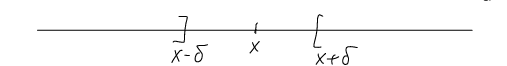
\includegraphics[0.5]{intervalleBoule.png}
       \end{center}
       

   \end{subparag} 
\end{parag}

\begin{parag}{Intérieur d'une boule}
    \begin{definition}
        Soit $E \subset \mathbb{R}^n $ non vide. Alors $ \overline{x} \in E$ est un \important{point intérieur} de $E$ s'il existe $ \delta > 0$ tel que $B( \overline{x}, \delta) \subset E$. L'ensemble des points intérieurs est appelé \important{intérieure} de $E$. Notation $ \mathring{E}$
    \end{definition}
   \begin{subparag}{Remarque personnelle}
       \begin{framedremark}
           On voit ici clairement que $ \mathring{E} < E$. Cette relation est vrai grâce au $ \delta$ qui rend \textit{"plus petit"} notre point $ \overline{x}$
       \end{framedremark}
   \end{subparag}
   Soit $E \subset \mathbb{R}^n $ non vide. Alors $E subset \mathbb{R}^n $ est ouvert $\iff E = \mathring{E}$
   \begin{subparag}{Exemple 1}
       La boule ouverte $B( \overline{x}, \delta) = \{ \overline{y} \in \mathbb{R}^n : \mid  \mid \overline{x} - \overline{y} \mid \mid < \delta \}$ est un sous-ensemble ouvert.\\
       Soit $ \overline{y} \in B( \overline{x}, \delta)$ Alors $ \delta = \frac{1}{2}( \delta - \mid  \mid x - y \mid \mid)  > 0$ implique que:
       \begin{align*}
         &\implies  B( \overline{y}_1, \delta_1) \subset B( \overline{x}, \delta) \\
         &\implies B( \overline{x}, \delta) \subset \mathbb{R}^n 
       \end{align*}
       est un sous-ensemble ouvert de $ \mathbb{R}^n $ $ \forall \overline{x} \in \mathbb{R}^n $, $ \forall \delta > 0$
   \end{subparag}
   \begin{subparag}{Exemple 2}
       Soit $n \geq 2$, $E = \{ \overline{x} \in \mathbb{R}^n  : x_1 = 0, x_i > 0, i = 2, \dots n\} \subset \mathbb{R}^n $
       Ici, nous voulons monter qu'il n'est pas ouvert. \\
       Prenons le point $ \overline{y} = (0, y_2, \dots, y_n)$ où $y_2, \dots, y_n > 0$. Alors pour tout $ \delta > 0$:
       \begin{align*}
           B( \overline{y}, \delta) \ni ( \frac{ \delta}{2}, y_2, \dots, y_n) \notin E
       \end{align*}
       
       
   \end{subparag}
   \begin{subparag}{Exemple 3}
       $\emptyset$ et $ \mathbb{R}^n  \subset \mathbb{R}^n $ sont des sous-ensembles ouverts.      \\
       Ici on a deux cas de figure, 
       \begin{itemize}
           \item $ emptyset$: alors le sous-ensemble est ouvert par définition
           \item Sinon, soit $ \overline{x} \in \mathbb{R}^n $ alors $B( \overline{x}, \delta) \subset \mathbb{R}^n $ et cela: $ \forall \delta > 0$
       \end{itemize}
   \end{subparag}
   \begin{subparag}{Exemple 4}
       $E = \{ \overline{x} \in \mathbb{R}^n: x_i > 0 \forall i = 1, \dots, n\}$\\
       Soit $ \overline{y} \in E$. Alors, nous pouvons prendre $B( \overline{y}, $min$(y_i)) \subset E$.
   \end{subparag}
\end{parag}

\begin{parag}{Propriétés}
    Ici on remarque deux grandes propriétés:
    \begin{enumerate}
       \item Toute réunion $\bigcup_{i \in I} E_i$ des sous-ensembles ouverts est un sous-ensemble ouvert.
           \begin{align*}
               \overline{x} \in \bigcup_{i \in I} E_i \implies \exists j: \overline{x} \in E_j, \; \; E_j \text{ est ouvert } \implies \exists \delta > 0: B( \overline{x}, \delta) \subset E_j \\
               \implies B( \overline{x}, \delta) \subset \bigcup_{i \in I}E_i
           \end{align*}
           

       \item Toute intersection \important{finie} $ \bigcap_{i=1}^nE_i$ des sous-ensembles ouverts est un sous-ensemble ouvert:
            \begin{align*}
               \overline{x} \in  \bigcap_{i\in I}E_i \implies \forall j \overline{x} \in E_j \text{ ouvert } \implies \exists \delta_j > 0 : B( \overline{x}, \delta_j) \subset E_j \\
               \implies B( \overline{x}, \text{min}_j \delta_j) \subset E_j \forall j \implies B( \overline{x}, \text{min} \delta_j) \subset \bigcap_{i=1}^n E_i = E
           \end{align*}
        
    \end{enumerate}
    \begin{framedremark}
        Une intersection infinie des sous-ensembles ouvert de $ \mathbb{R}^n $
    \end{framedremark}
    
\end{parag}



\begin{parag}{Sous-ensemble fermé}
    \begin{definition}
        Soit $E \subset \mathbb{R}^n$ un sous-ensemble. Alors $E$ est \important{Fermé} dans $ \mathbb{R}^n$ si son complément $CE = \{ \overline{x} \in \mathbb{R}^n : \overline{x} \notin E\} = \mathbb{R}^n - E$ est ouvert
    \end{definition}
    
        \begin{align*}
            CB( \overline{x}, \delta) = E \subset \mathbb{R}^n \text{ est fermé}: E = \{ \overline{y} \in \mathbb{R}^n : \mid  \overline{x} - y \mid \geq \delta \} 
        \end{align*}
            Puisque $C(CB( \overline{x}, \delta)) = B( \overline{x}, \delta)$ est ouvert.
\end{parag}
\begin{parag}{Exemples}
    \begin{align*}
        E = \{ \overline{x}\} \subset \mathbb{R}^n 
    \end{align*}
    Ceci est \important{fermé}, car si on prends le complément:
    \begin{align*}
        CE = \{ \overline{y} \in \mathbb{R}^n : \mid \mid \overline{y} - \overline{x} \mid \mid > 0\} \\
        \forall \overline{y} \in CE\; \; \text{la boule} \overline{B}( \overline{y}, \frac{1}{2} \mid  \mid \overline{y} - \overline{x} \mid \mid \subset CE
    \end{align*}
    
    

\end{parag}

\begin{parag}{Question pendant le cours}
    Soient $A$ et $B$ deux sous-ensembles ouverts non-vides de $ \mathbb{R}^n $ Soit $A \setminus B = \{ \overline{x} \in \mathbb{R}^n : \overline{x} \in A \text{ et } \overline{x} \notin B\} $ non-vide.
    \begin{enumerate}
        $A \setminus B$ peut être ouvert, fermé ou ni ouvert ni fermé
        \item $A \setminus$ est soit ouvert, soit fermé
        \item $A \setminus$ ne peut pas être ouvert
        \item $A \setminus$ ne peut pas être fermé
    \end{enumerate}
    Il n'y a qu'une seul possibilité et pour la trouver il faut des contre exemples.

\end{parag}
\begin{parag}{Exemple}
    \begin{align*}
        A = \{(x, y) \in \mathbb{R}^2 : \tan(x + y) \geq 1\}
    \end{align*}
    Et on se pose la question $A$ ouvert, fermé, ni ouvert, ni fermé?
    \\
    Déjà on va trouver tout les valeurs possiblie pour $x$ et $y$ c'est à dire la définition de $\tan$:
    \begin{align*}
        \implies \tan u \text{ existe } \implies u \in ] - \frac{ \pi}{2} + \pi k, \frac{\pi}{2} + \pi k[ \; k \in \mathbb{Z} \\
        \tan u \geq 1 \implies u \in [ \frac{\pi}{4} + \pi k, \frac{\pi}{2} + \pi k[ \; \; \forall k \in \mathbb{Z}
    \end{align*}
   On a donc comme dit auparavant:
   \begin{align*}
       x + y \in  [ \frac{\pi}{4} + \pi k, \frac{\pi}{2} + \pi k[\\
       \frac{\pi}{4} + \pi k \leq x + y < \frac{\pi}{2} + \pi k, k \in \mathbb{Z}\\
       \frac{\pi}{4} + \pi k - x \leq y < \frac{\pi}{2} + \pi k -x
   \end{align*}
   Ici $A$ n'est ni ouvert ni fermé:
   \begin{center}
       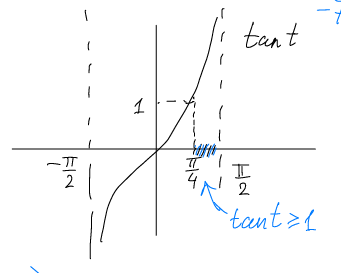
\includegraphics[0.6]{tanBoule.png}
   \end{center}
   \textbf{Explications}: \\
   \begin{enumerate}
       \item $A$ n'est pas ouvert: $(x, y) = (0, \frac{\pi}{4}) = p \in A$
       \begin{align*}
           \forall \delta > 0 \; \; B( \overline{p}, \delta) \text{ contient } (0, \frac{\pi}{4} - \frac{ \delta}{2}) \notin A
       \end{align*}
   \item $A$ n'est pas fermé: $(x, y) = (0, \frac{\pi}{2}) = q \in CA$ 
       \begin{align*}
           \forall \delta > 0 B( \overline{q}, \delta) \text{ contient } (0, \frac{\pi}{2}- \frac{ \delta}{2}) \in A \implies (0, \frac{\pi}{2} - \frac{ \delta}{2}) \notin CA
       \end{align*}
       Et comme $CA$ n'est pas ouvert, alors $A$ n'est pas fermé.
   \end{enumerate}
\end{parag}

\subsection{Méthodes de démonstration: Démonstration par le principe des tiroirs}
\begin{parag}{Principes des tiroirs}
    Si $(n+1)$ objets sont placés dans $n$ tiroirs, alors au moins un tiroir contient $2$ objets ou plus.
    \\
    Plus généralement:
    \begin{theoreme}
        Si $n$ objets sont placés dans $k$ tiroirs, alors au moins un tiroir contient $\left\ceiling \frac{n}{k} \right\ceiling = $min$\{m \in \mathbb{N}: m \geq \frac{n}{k}\}$ objets, ou plus.
    \end{theoreme}
    
    \begin{framedremark}
        Ceci est exactement la même méthode que celle vu en AICC I qu'on appelait le pigeon hole principle, Les preuves sont exactement les mêmes est le but est exactement le même.
    \end{framedremark}
    
\end{parag}

